\documentclass{article} 

\usepackage[utf8]{inputenc}
\usepackage{amssymb,amsmath}

\usepackage{graphicx}

\usepackage[top=3cm, bottom=3cm, left=3cm, right=3cm, includefoot]{geometry}

\usepackage{amsthm}
\theoremstyle{lemma}
\newtheorem{lemma}{Lemma}


\begin{document}

Let us consider the set of $m$ points
\begin{displaymath}
 \mathcal{P} = \lbrace p_1, \dots, p_m \rbrace \subset \mathbb{R}^d ~\mathrm{.}
\end{displaymath}
The problem is to find a center of ball such that the maximum distance between this center and points in $\mathcal{P}$ is minimal, i.e.
\begin{equation}
 \label{eq:ball_problem}
 \bar{p} := \underset{p}{\arg} \min\limits_{p \in \mathbb{R}^d} \lbrace \max\limits_{p_i \in \mathcal{P}} \Vert p_i - p \Vert  \rbrace ~\mathrm{,}
\end{equation}
and the radius of this ball is given by the value of maximum distance between the center and points from $\mathcal{P}$, i.e.
\begin{displaymath}
 r := \max\limits_{p_i \in \mathcal{P}} \Vert p_i - p \Vert ~\mathrm{.}
\end{displaymath}
Similarly to \emph{polytope example (test 03)}, we will search for a coeficient vector of the convex linear combination 
\begin{displaymath}
 p = \sum\limits_{i = 1}^{m} \alpha_{i} p_i, ~ \mathrm{where} ~ \sum\limits_{i = 1}^{m} \alpha_i = 1 ~ \mathrm{and} ~ 0 \leq \alpha_i \leq 1 ~\forall i = 1,\dots,m  ~\mathrm{.}
\end{displaymath}
The reason is that the center of enclosing ball lies in the convex hull of $\mathcal{P}$ (see Sch\"{o}nherr). \newline
Afterwards, we denote
\begin{displaymath}
 \begin{array}{rcl}
  y & := & [\alpha_1, \dots, \alpha_m]^T \in \mathbb{R}^{m} ~\mathrm{,} \\
  C & := & [p_1,\dots,p_m] \in \mathbb{R}^{d,m} ~\mathrm{,} \\
  b & := & [p_1^T p_1, \dots, p_m^T p_m]  \in \mathbb{R}^{m} ~\mathrm{.} 
 \end{array}
\end{displaymath}
The problem \eqref{eq:ball_problem} can be reformulated to QP. See next lemma.
\begin{lemma}
The solution of optimization problem
\begin{displaymath}
 \bar{p} := C\bar{y}, ~~~~ \bar{y} := \arg \min\limits_{y \in \Omega_E \cap \Omega_I} y^T C^T C y - b^T C y,
\end{displaymath}
where
\begin{displaymath}
 \begin{array}{rcl}
  \Omega_E & := & \left\lbrace y \in \mathbb{R}^{m}: B x = 1 \right\rbrace ~\mathrm{,} \\
  \Omega_I & := & \left\lbrace y \in \mathbb{R}^{m}: x \geq 0 \right\rbrace ~\mathrm{,} \\
  B & := & [1,\dots,1] \in \mathbb{R}^{1,m} \\
 \end{array}
\end{displaymath}
is equivalent to the solution of the problem \eqref{eq:ball_problem}.
\end{lemma}

\begin{proof}
See Sch\"{o}nherr 
%\cite{SchPHD-2002}
. The proof is based on KKT optimality conditions.
\end{proof}

Moreover, the problem can be homogenized and solved using the same methodology as in \emph{polytope example (test 03)}.
We solve the problem to obtain the center of ball $\bar{p}$. Afterwards, the radius can be computed by
\begin{displaymath}
 r = \sqrt{-\bar{p}^T A\bar{p} + 2 b^T \bar{p}} ~\mathrm{.}
\end{displaymath}

%\clearpage

\paragraph{Numerical example}

We work with random data in our benchmark. We generate $m = 100$ random points from circle
\begin{displaymath}
 \lbrace p \in \mathbb{R}^2: \Vert p - [1, 1]^T \Vert^2 \leq 1 \rbrace. 
\end{displaymath}
Afterwards, we discard the information about the circle and try to find the enclosing ball using the process described above.

\begin{figure}[h!]
\begin{center}
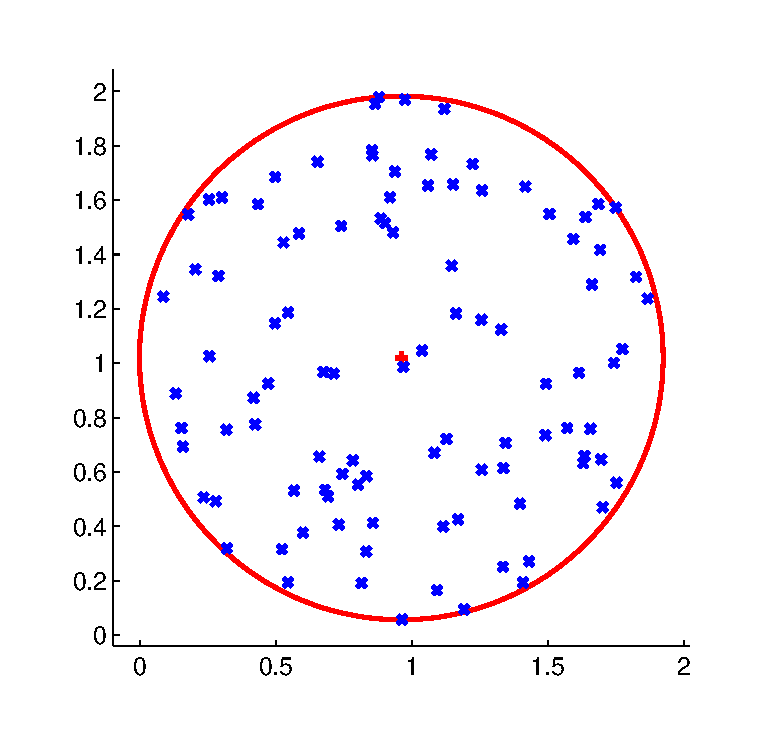
\includegraphics[width=0.37\textwidth]{ball_solution.eps}
\caption[Enclosing ball: the solution of benchmark]{Enclosing ball: the solution of the benchmark.}
\label{fig:ball_solution}
\end{center}
\end{figure}


\end{document}

